\documentclass[a4paper,
fontsize=11pt,
%headings=small,
oneside,
numbers=noperiodatend,
parskip=half-,
bibliography=totoc,
final
]{scrartcl}

\usepackage{synttree}
\usepackage{graphicx}
\setkeys{Gin}{width=.4\textwidth} %default pics size

\graphicspath{{./plots/}}
\usepackage[ngerman]{babel}
\usepackage[T1]{fontenc}
%\usepackage{amsmath}
\usepackage[utf8x]{inputenc}
\usepackage [hyphens]{url}
\usepackage{booktabs} 
\usepackage[left=2.4cm,right=2.4cm,top=2.3cm,bottom=2cm,includeheadfoot]{geometry}
\usepackage{eurosym}
\usepackage{multirow}
\usepackage[ngerman]{varioref}
\setcapindent{1em}
\renewcommand{\labelitemi}{--}
\usepackage{paralist}
\usepackage{pdfpages}
\usepackage{lscape}
\usepackage{float}
\usepackage{acronym}
\usepackage{eurosym}
\usepackage[babel]{csquotes}
\usepackage{longtable,lscape}
\usepackage{mathpazo}
\usepackage[normalem]{ulem} %emphasize weiterhin kursiv
\usepackage[flushmargin,ragged]{footmisc} % left align footnote
\usepackage{ccicons} 
\setcapindent{0pt}

%%%% fancy LIBREAS URL color 
\usepackage{xcolor}
\definecolor{libreas}{RGB}{112,0,0}

\usepackage{listings}

\urlstyle{same}  % don't use monospace font for urls

\usepackage[fleqn]{amsmath}

%adjust fontsize for part

\usepackage{sectsty}
\partfont{\large}

%Das BibTeX-Zeichen mit \BibTeX setzen:
\def\symbol#1{\char #1\relax}
\def\bsl{{\tt\symbol{'134}}}
\def\BibTeX{{\rm B\kern-.05em{\sc i\kern-.025em b}\kern-.08em
    T\kern-.1667em\lower.7ex\hbox{E}\kern-.125emX}}

\usepackage{fancyhdr}
\fancyhf{}
\pagestyle{fancyplain}
\fancyhead[R]{\thepage}

% make sure bookmarks are created eventough sections are not numbered!
% uncommend if sections are numbered (bookmarks created by default)
\makeatletter
\renewcommand\@seccntformat[1]{}
\makeatother


\usepackage{hyperxmp}
\usepackage[colorlinks, linkcolor=black,citecolor=black, urlcolor=libreas,
breaklinks= true,bookmarks=true,bookmarksopen=true]{hyperref}
\usepackage{breakurl}

%meta
%meta

\fancyhead[L]{K. Schlebbe\\ %author
LIBREAS. Library Ideas, 34 (2018). % journal, issue, volume.
\href{http://nbn-resolving.de/}
{}} % urn 
% recommended use
%\href{http://nbn-resolving.de/}{\color{black}{urn:nbn:de...}}
\fancyhead[R]{\thepage} %page number
\fancyfoot[L] {\ccLogo \ccAttribution\ \href{https://creativecommons.org/licenses/by/4.0/}{\color{black}Creative Commons BY 4.0}}  %licence
\fancyfoot[R] {ISSN: 1860-7950}

\title{\LARGE{Ein Jubiläum kommt selten allein: 20 Jahre Berliner Bibliothekswissenschaftliches Kolloquium}}% title
\author{Kirsten Schlebbe} % author

\setcounter{page}{1}

\hypersetup{%
      pdftitle={Ein Jubiläum kommt selten allein: 20 Jahre Berliner Bibliothekswissenschaftliches Kolloquium},
      pdfauthor={Kirsten Schlebbe},
      pdfcopyright={CC BY 4.0 International},
      pdfsubject={LIBREAS. Library Ideas, 34 (2018).},
      pdfkeywords={Bibliothekswissenschaft, Institut für Bibliotheks- und Informationswissenschaft, Humboldt-Universität zu Berlin, Berliner Bibliothekswissenschaftliches Kolloquium, BBK},
      pdflicenseurl={https://creativecommons.org/licenses/by/4.0/},
      pdfcontacturl={http://libreas.eu},
      baseurl={http://libreas.eu},
      pdflang={de},
      pdfmetalang={de}
     }



\date{}
\begin{document}

\maketitle
\thispagestyle{fancyplain} 

%abstracts

%body
\hypertarget{hintergrund}{%
\section{Hintergrund}\label{hintergrund}}

Eine Anfrage von Studierenden der Staatlichen Universität für Kunst und
Kultur in St.~Petersburg machte uns im Dezember 2017 darauf aufmerksam,
dass nicht nur das Institut für Bibliotheks- und
Informationswissenschaft (IBI) im Jahr 2018 ein Jubiläum begeht. Ein
Blick in die Aufzeichnungen sowie das Gespräch mit aktuellen und
ehemaligen Mitarbeitenden zeigte, dass auch eine andere Institution im
Januar diesen Jahres einen runden Geburtstag feiern konnte: Das Berliner
Bibliothekswissenschaftliche Kolloquium (BBK) existiert als
Vortragsreihe am Institut für Bibliotheks- und Informationswissenschaft
seit nunmehr 20 Jahren.

Auf Anregung von Michael Heinz, der fachliche Kolloquien während seiner
Zeit am Institut für Mathematik an der Humboldt-Universität
kennengelernt hatte, und unter der Leitung des damaligen
geschäftsführenden Direktors Prof.~Dr.~Robert Funk, wurde das Kolloquium
im Wintersemester 1997/98 ins Leben gerufen. Eine Einladung (Abb. 1)
erinnert an den ersten Termin am Dienstag, dem 20. Januar 1998.

\begin{figure}
\centering
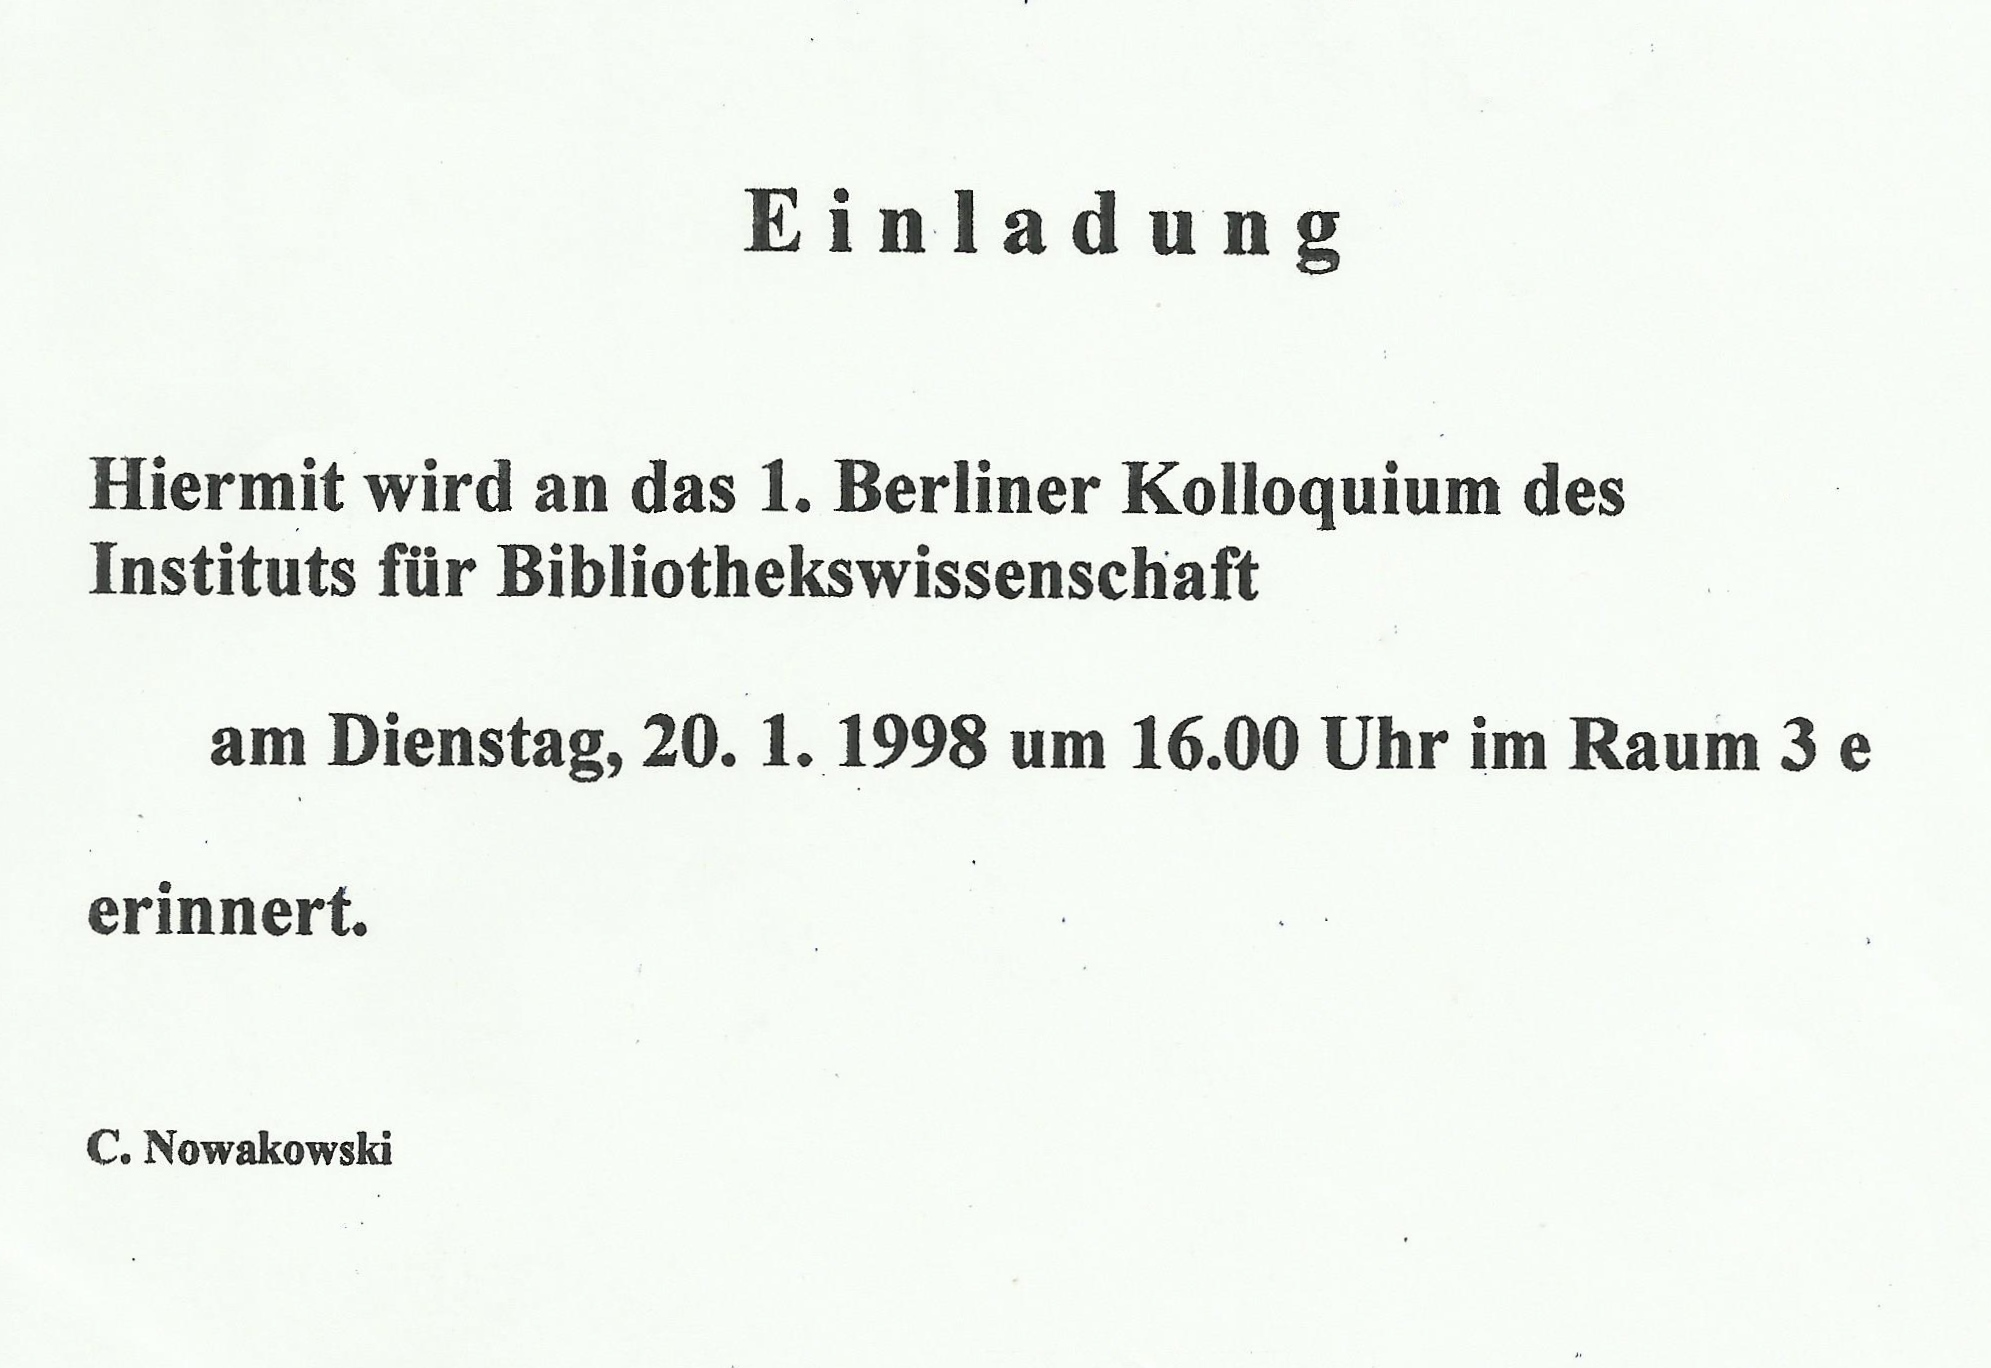
\includegraphics[width=10cm]{img/Abbildung1.jpg}
\caption{Einladung zum ersten BBK am 20.01.1998 (Quelle: Privatarchiv
Dr.~Gertrud Pannier)}
\end{figure}

Hintergrund für die Idee einer institutseigenen Veranstaltungsreihe war
nach Aussage von Michael Heinz \enquote{einerseits das Bedürfnis, die
Kommunikation sowohl unter den Professoren und wissenschaftlichen
Mitarbeitern zu verbessern {[}\ldots{}{]}. Andererseits war das Anliegen, die
Kontakte mit der Praxis auszubauen und die eigene Forschung stärker
sichtbar zu machen {[}\ldots{}{]} eine Kommunikationsplattform zu
schaffen, die der eigenen Weiterbildung genauso dient, wie der
Information untereinander, mit Studierenden und der bibliothekarischen
und informatorischen Praxis. {[}\ldots{}{]} Bei der Zeitplanung wurde
ausdrücklich beachtet, dass ein geeigneter Wochentag und eine günstige
Uhrzeit die Teilnahme des im Berliner und Potsdamer Raum reichlich
vorhandenen Fachpersonals weitestgehend ermöglichen sollen.
{[}\ldots{}{]} Und es war klar, dass ein verlässlicher wöchentlicher
Rhythmus in den Semestermonaten gewährleistet werden musste, um diese
Veranstaltungsreihe zu etablieren.} (Dr.~Gertrud Pannier, persönliche
Korrespondenz, 08.12.2017).

Bis zum heutigen Tag findet das BBK während der Semestermonate dienstags
am frühen Abend statt. Die Leitung des Kolloquiums liegt in der Regel
bei den DirektorInnen des Instituts. Die praktische Organisation wurde
zum einen von wissenschaftlichen MitarbeiterInnen und seit 2011 auch von
einer eigenen studentischen Hilfskraft für das BBK übernommen. Bereits
seit dem Beginn der Reihe wurden die Termine online verzeichnet und zum
Teil wurden zusätzliche Materialien wie Abstracts, Vortragsfolien oder
Volltexte verlinkt. Seit 2011 gab es auch erste Audio- und
Videoaufzeichnungen der Vorträge. Mittlerweile werden die Aufnahmen
standardmäßig über das Medienrepositorium der Humboldt-Universität und
Verlinkungen auf der Webseite des BBK\footnote{\href{http://www.ibi.hu-berlin.de/de/bbk}{http://www.ibi.hu-berlin.de/de/bbk}}
zur Verfügung gestellt.

Während bei dem ersten Termin im Januar 1998 im Rahmen einer Gründungs-
und Diskussionsveranstaltung eher institutsinterne Fragen erläutert
werden sollten, sind die nachfolgenden Termine (27.01.1998 -- heute) auf
den aktuellen sowie archivierten Webseiten des Institutes verzeichnet
und bis heute einsehbar.\footnote{Siehe die BBK-Websites
  \url{https://www.ibi.hu-berlin.de/de/bbk/bbk-archiv} (Sommersemester
  2007 bis heute) sowie
  \url{http://www.ib.hu-berlin.de/about/veranst/bbk/index.html}
  (Sommersemester 2005 bis Wintersemester 2006/07) und
  \url{http://www.ib.hu-berlin.de/about/veranst/bbk/archiv/index.html}
  (Wintersemester 1998 bis Wintersemester 2004/2005) {[}zuletzt
  abgerufen am 3.10.2018{]}}

Für den vorliegenden Artikel wurden die BBK-Termine zwischen dem
27.01.1998 bis zum 10.07. 2018 mit ihren charakteristischen Daten (Datum,
Titel, ReferentIn sowie Institution) zusammengetragen, bereinigt und
ausgewertet.\footnote{Eine tabellarische Übersicht der BBK-Termine sowie
  weitere Statistiken sind als (Roh-)Datendokumente im XLSX-Format dem
  Artikel als Supplement beigefügt, vgl. \enquote{BBK-Veranstaltungen (01/1998-07/2018)} \href{https://doi.org/10.18452/19506}{https://doi.org/10.18452/19506} bzw. \enquote{Materialien zur Statistik des Berliner Bibliothekswissenschaftlichen Kolloquiums (BBK)} \href{https://doi.org/10.18452/19507}{https://doi.org/10.18452/19507}.} Die folgenden Absätze geben somit
einen Überblick über 20 Jahre Berliner Bibliothekswissenschaftliches
Kolloquium am Institut für Bibliotheks- und Informationswissenschaft und
bieten auf diese Weise auch einen Einblick in die Entwicklung der
Forschung und Ausrichtung des Instituts und seiner jeweiligen
Mitarbeitenden.

In einem ersten Schritt werden die Anzahl der Vorträge insgesamt sowie
die Entwicklung der Zahlen über die Semester erläutert. Im Anschluss
sollen die ReferentInnen des BBKs näher betrachtet werden: Wie viele
Personen waren im Schnitt an einem Vortrag beteiligt und welche Person
war an den meisten Vorträgen beteiligt? Weiterhin wird ein kritischer
Blick auf das Geschlechterverhältnis bei den Vortragenden im BBK
geworfen. Auch die Frage nach dem Verhältnis von \enquote{IBI-internen}
und externen ReferentInnen wird gestellt. Die Analyse schließt mit einem
Blick auf die Entwicklung der behandelten Themenfelder.

\hypertarget{ergebnisse}{%
\section{Ergebnisse}\label{ergebnisse}}

\hypertarget{anzahl-der-vortruxe4ge}{%
\subsection{Anzahl der Vorträge}\label{anzahl-der-vortruxe4ge}}

Zwischen dem 27.01.1998 und dem 10.07.2018 wurden im Verlauf von 42
Semestern insgesamt 476 Vorträge gehalten. Abbildung 2 zeigt, dass die
Anzahl der Vorträge pro Semester dabei bis auf wenige Ausnahmen in den
ersten Jahren einigermaßen konstant blieb und dass in den längeren
Wintersemestern (blau) naturgemäß mehr Vorträge stattfanden als in den
kürzeren Sommersemestern (orange).

\begin{figure}[h!]
\centering
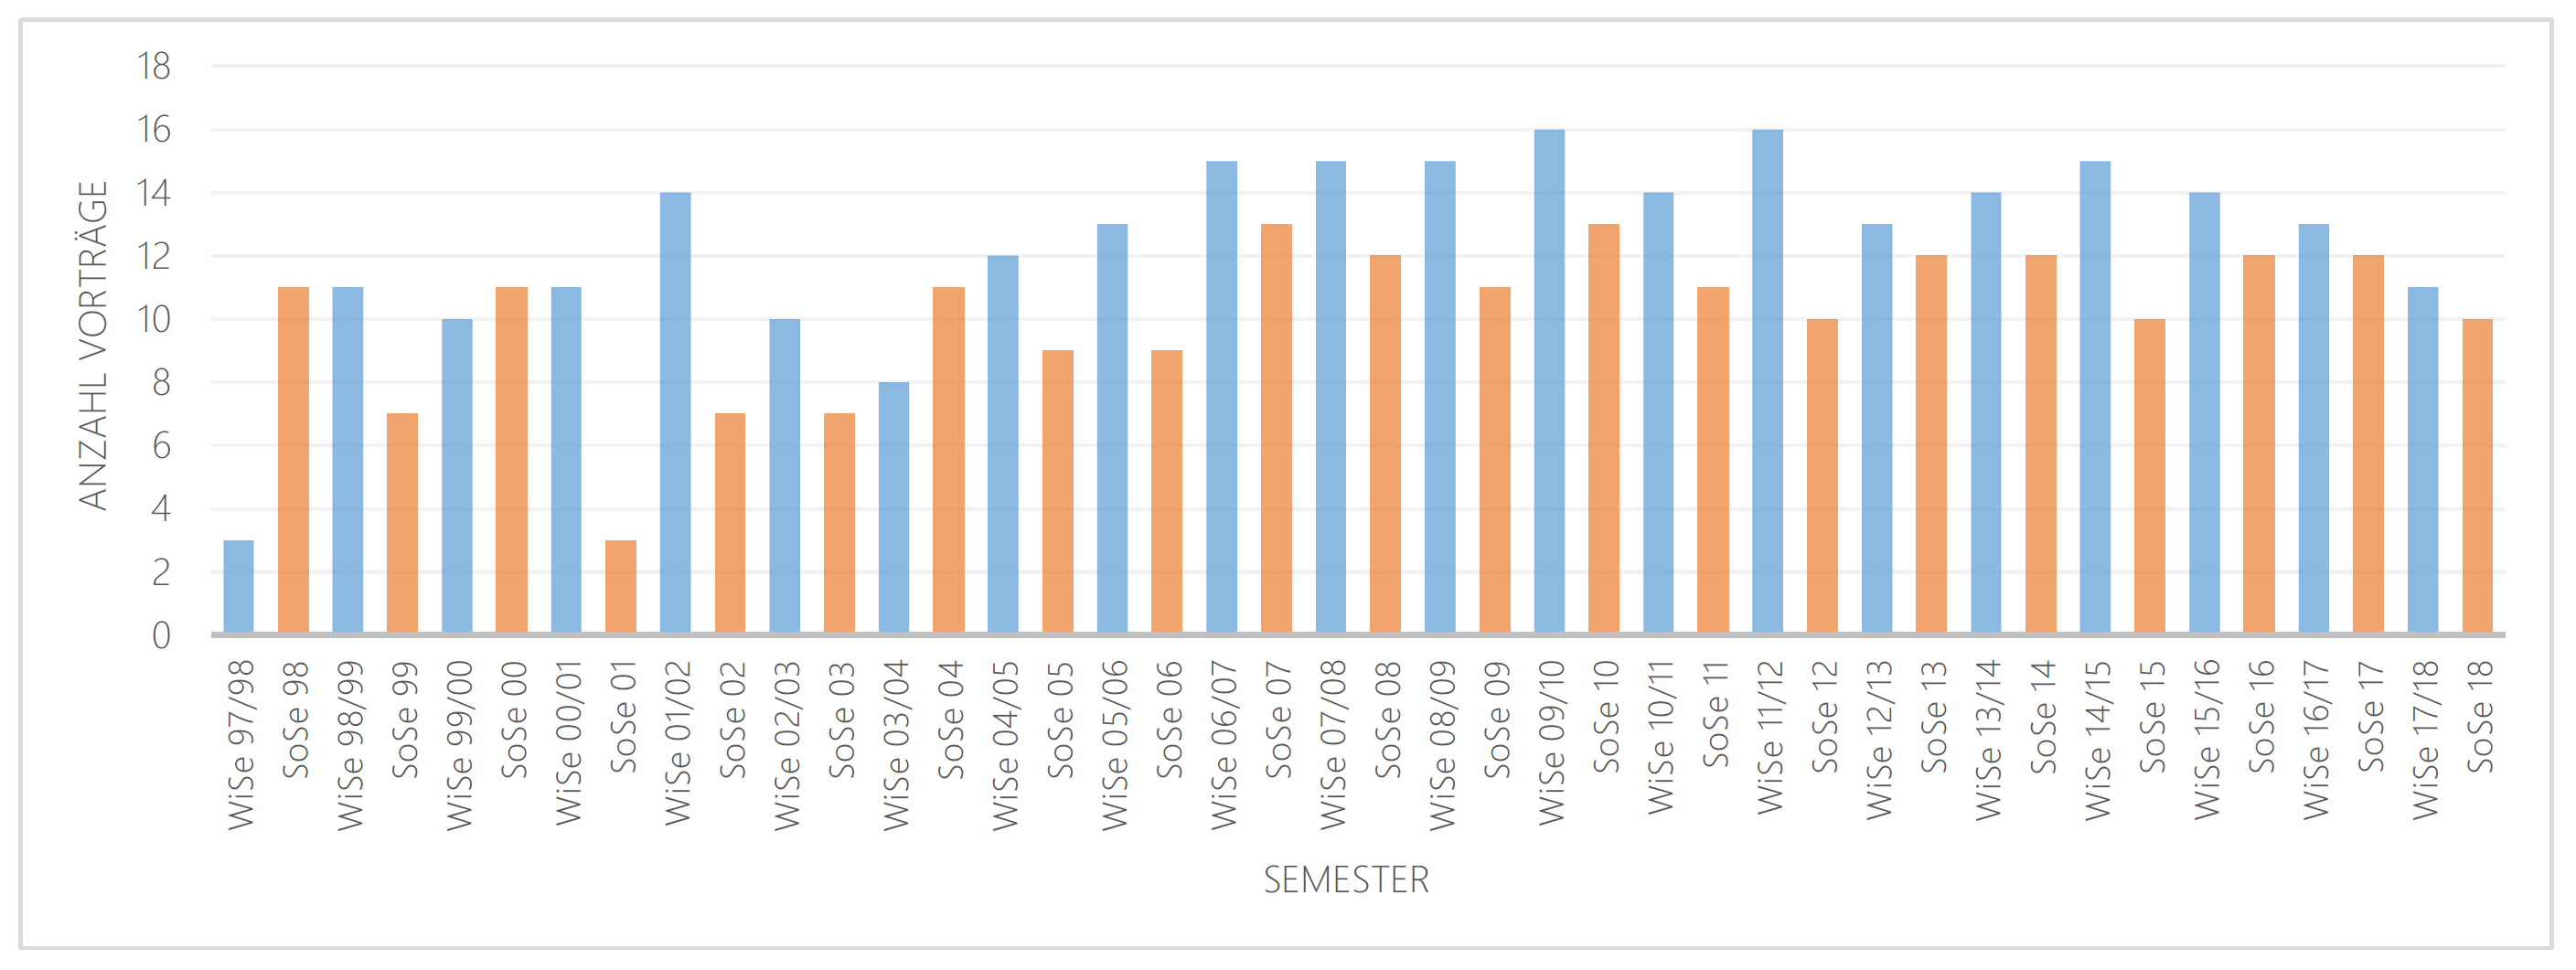
\includegraphics[width=16cm]{img/Abbildung2.png}
\caption{Anzahl der Vorträge pro Semester}
\end{figure}

\hypertarget{referentinnen}{%
\subsection{ReferentInnen}\label{referentinnen}}

\hypertarget{anzahl-der-referentinnen-pro-vortrag}{%
\subsubsection{Anzahl der ReferentInnen pro
Vortrag}\label{anzahl-der-referentinnen-pro-vortrag}}

Der klassische BBK-Vortrag wurde von einer einzelnen Person gehalten:
Bei 380 von 476 Vorträgen (79,83\,\%) ist ein/e einzelne/r ReferentIn
aufgeführt. Bei 59 Vorträgen (12,39\,\%) referierten zwei Personen, bei
12 Vorträgen (2,52\,\%) gab es drei ReferentInnen. Nur selten gab es vier
(4 mal; 0,84\,\%) oder fünf (2 mal; 0,42\,\%) Vortragende. Bei 19 Terminen
(3,99\,\%) bleibt die genaue Anzahl der ReferentInnen unklar, da es sich
um Diskussionsveranstaltungen handelt oder die ReferentInnen nicht alle
namentlich benannt sind (Beispielsweise Person X und Studierende).
Abbildung 3 zeigt die Verteilung in der Übersicht.

\begin{figure}[h!]
\centering
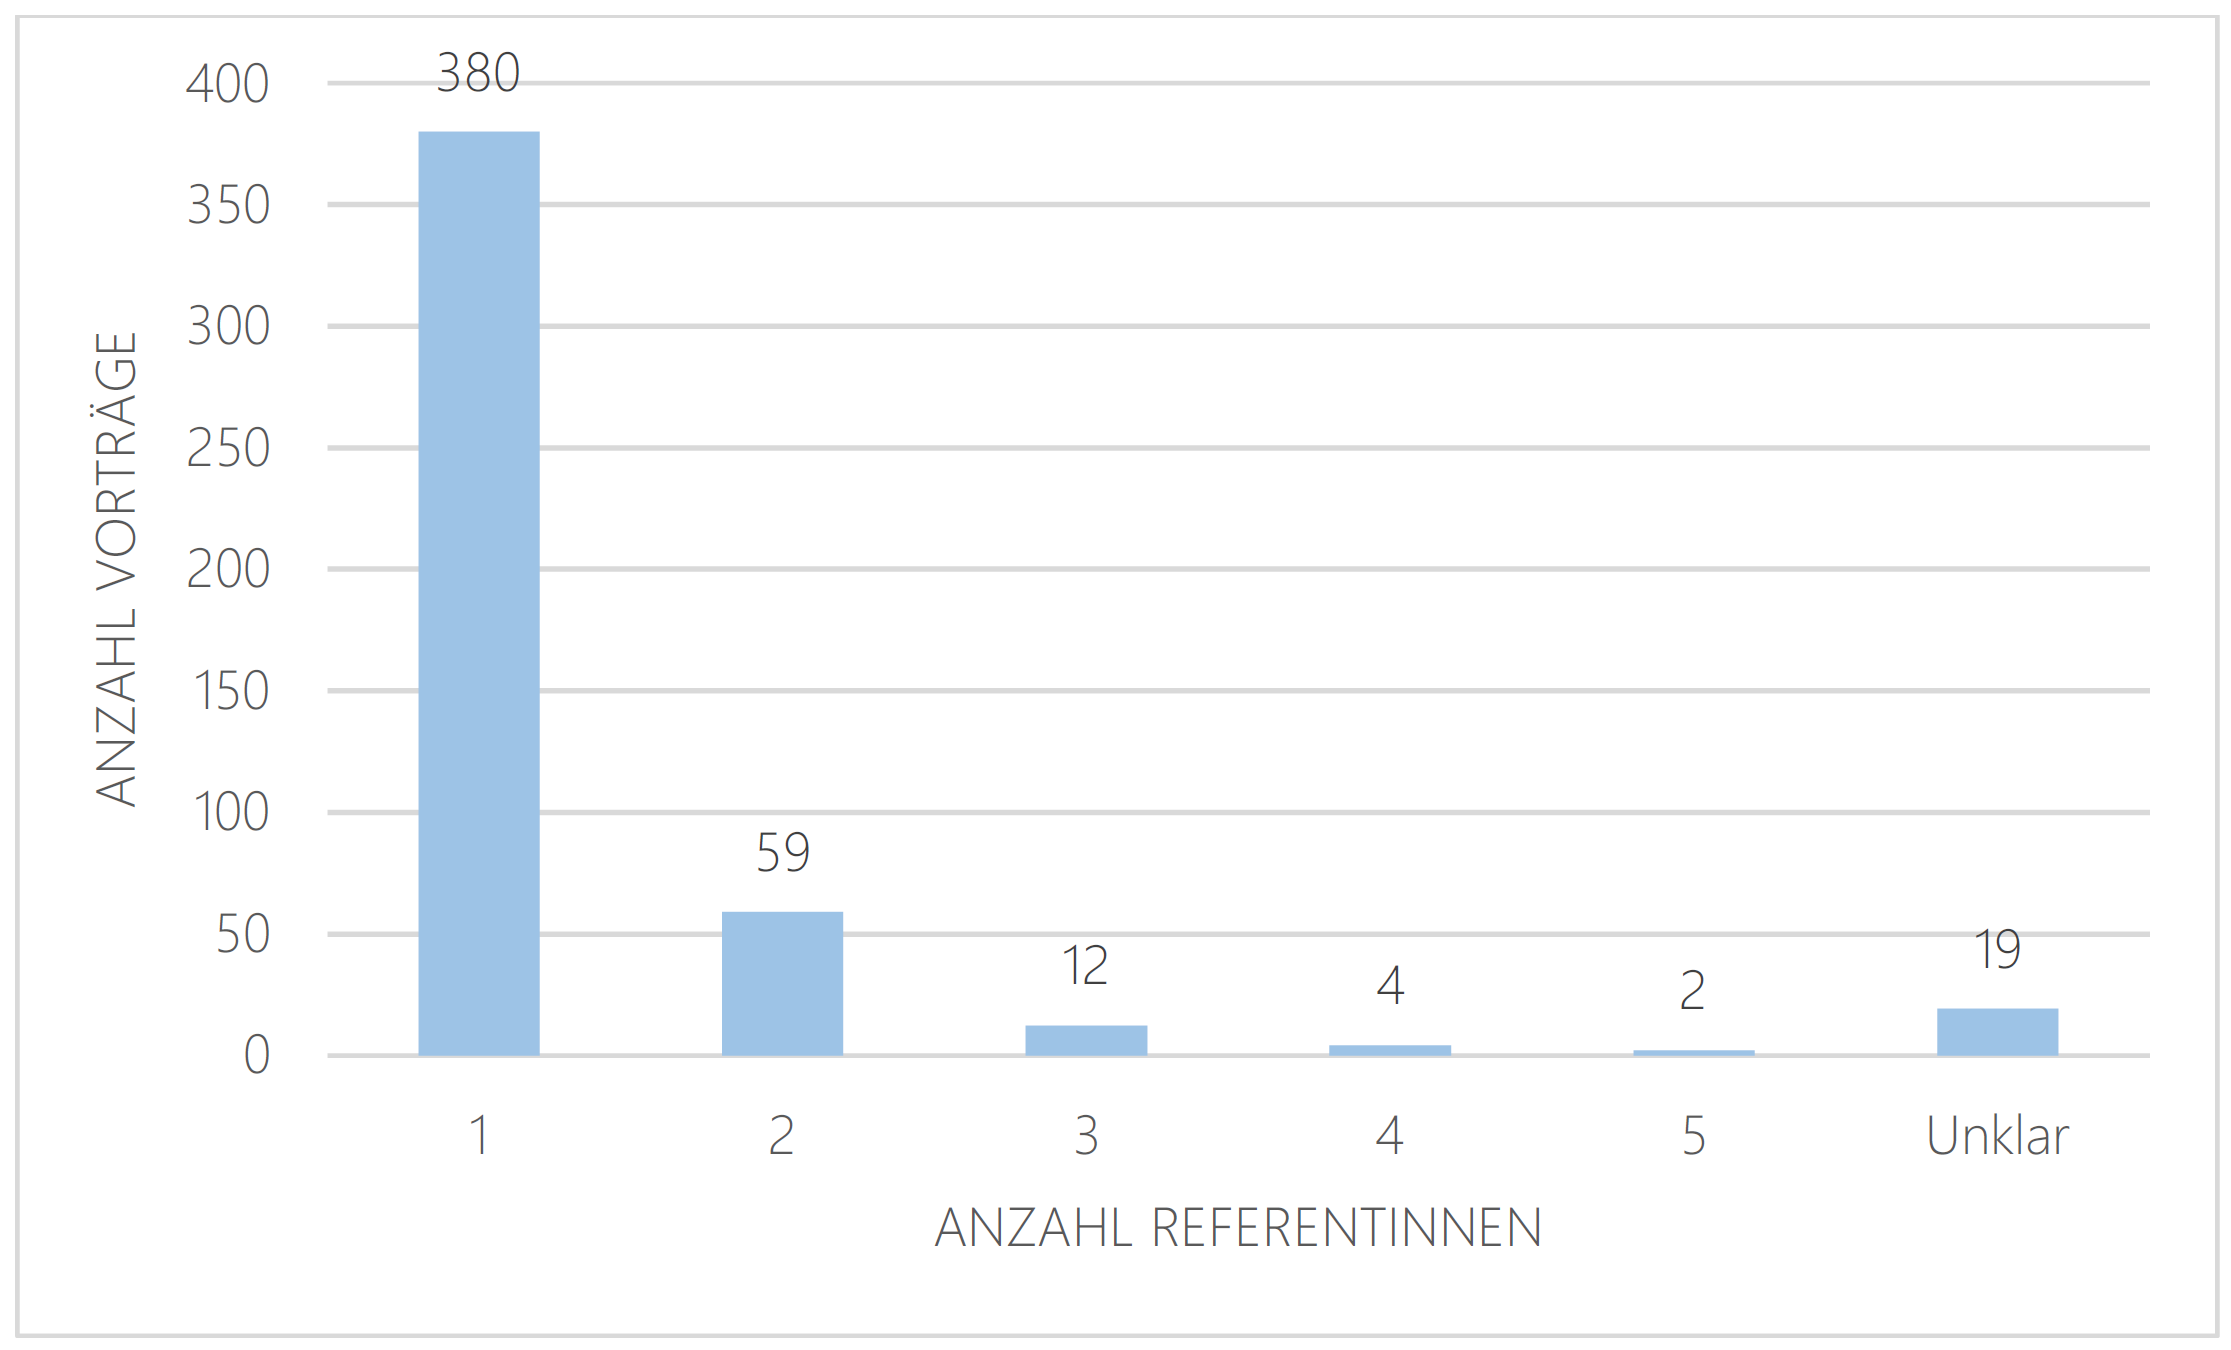
\includegraphics[width=12cm]{img/Abbildung3.png}
\caption{Anzahl der ReferentInnen pro Vortrag}
\end{figure}

Bei der Anzahl von ReferentInnen pro Vortrag zeigt sich auch im Verlauf
der Jahre keine große Veränderung. Der \enquote{Trend zum Kollektiv} in
der Wissenschaft (FAZ, 07.06.2018) kann also im Zusammenhang mit dem BBK
nicht bestätigt werden. Abbildung 4 bildet die Mittelwerte (Anzahl
ReferentInnen / Vortrag) für die einzelnen Semester ab.

\begin{figure}[h!]
\centering
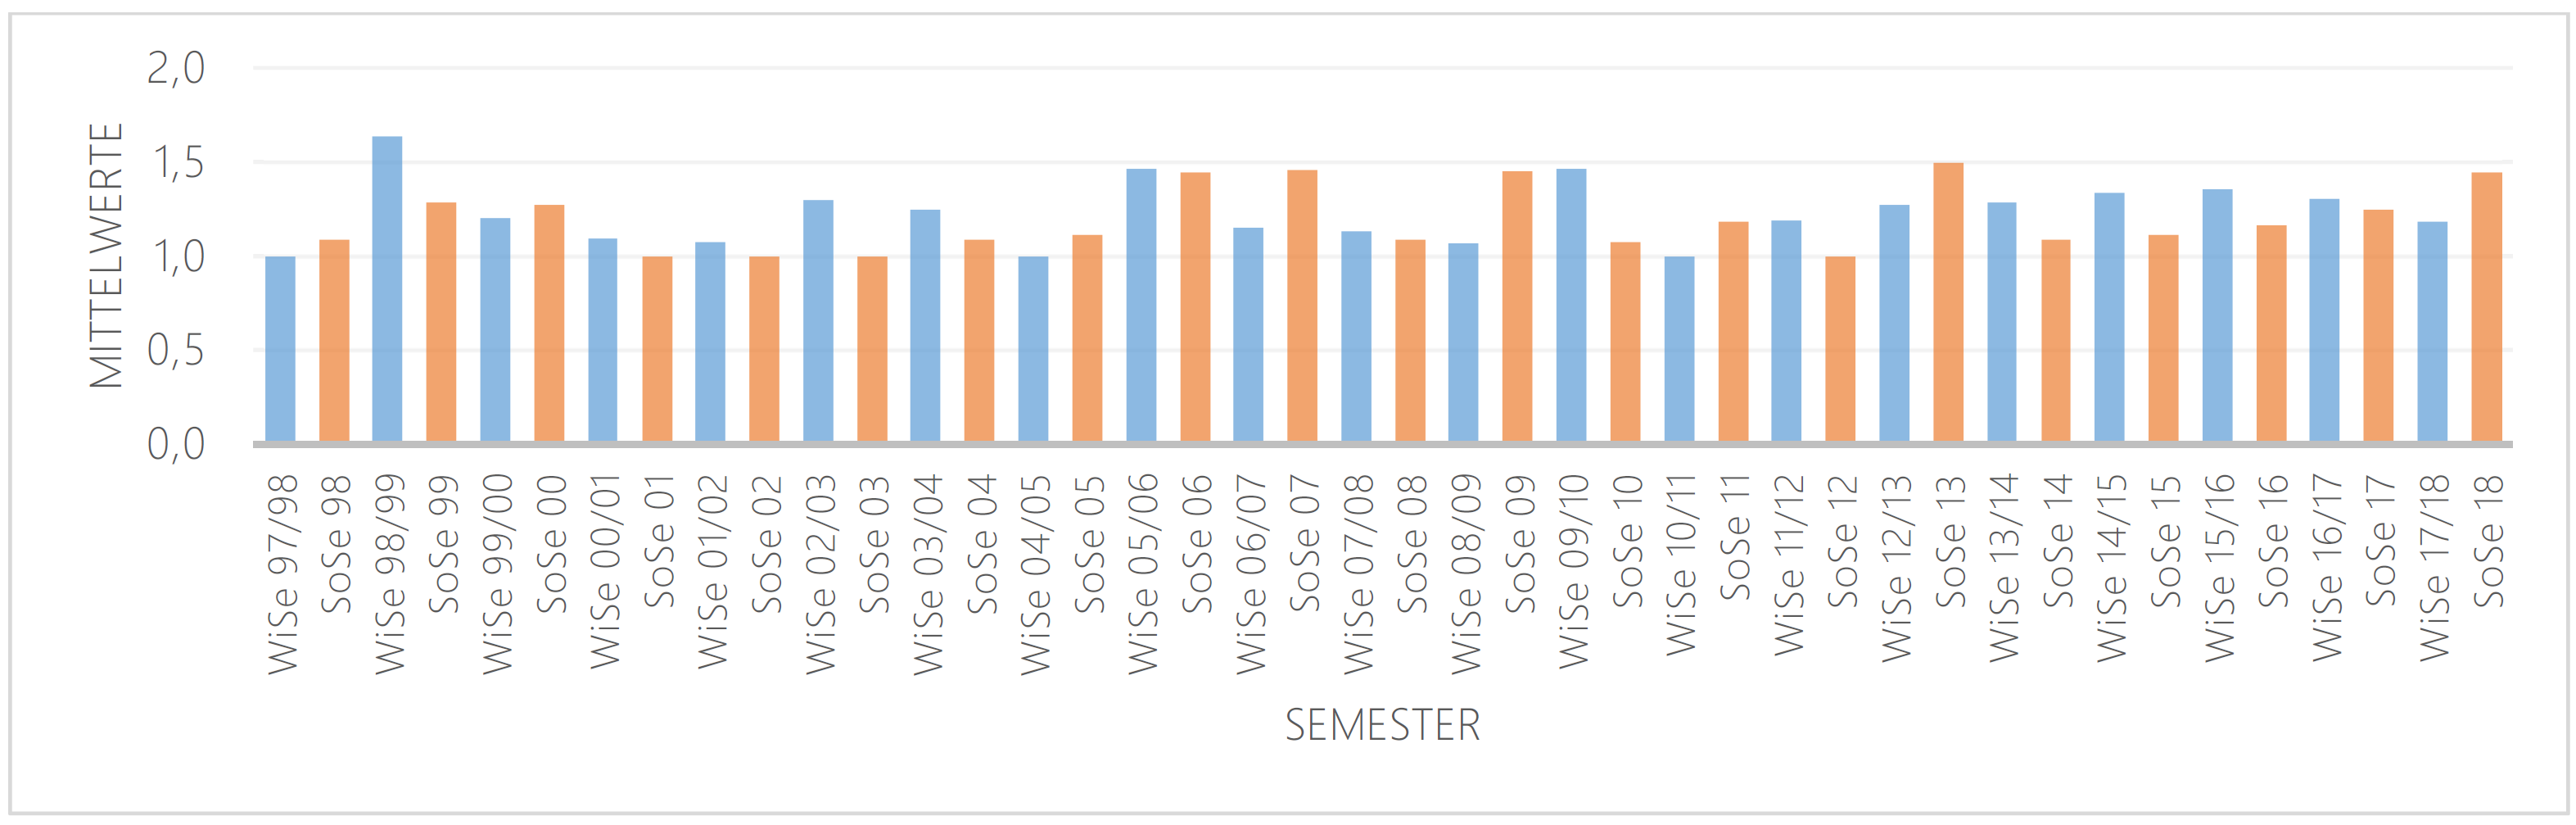
\includegraphics[width=16cm]{img/Abbildung4.png}
\caption{Mittelwerte für die Anzahl der ReferentInnen pro Vortrag pro
Semester}
\end{figure}

\hypertarget{anzahl-der-vortruxe4ge-pro-referentin}{%
\subsubsection{Anzahl der Vorträge pro
ReferentIn}\label{anzahl-der-vortruxe4ge-pro-referentin}}

Insgesamt waren 560 Vortragende an 457 Kolloquien beteiligt. Die oben
bereits angesprochenen 19 Termine, bei denen die genaue Anzahl an
ReferentInnen nicht ermittelt werden konnte, wurden von der folgenden
Analyse ausgeschlossen. Die 560 Vortragenden stellen jedoch nicht 560
verschiedene Personen dar: Durch mehrere Vorträge im BBK kam es zur
Mehrfachnennung von einigen Personen. Rechnet man diese heraus, so waren
von 1998 bis 2018 371 verschiedene Personen als Vortragende am BBK
beteiligt.\footnote{Nicht vollständig ausgeschlossen werden kann, dass
  Personen durch eine Namensänderung nach einer Eheschließung bei der
  Analyse als zwei verschiedene Personen gewertet wurden.} Dabei waren
33 Personen an zwei Vorträgen im BBK beteiligt, 13 Personen an drei
Vorträgen und sieben Personen waren bei vier Kolloquien als ReferentIn
aufgeführt. Die \enquote{Spitzenreiter} unter den ReferentInnen mit fünf
oder mehr Beteiligungen werden in Tabelle 1 aufgeführt. Mit großem
Abstand führt hierbei Prof.~Dr.~Konrad Umlauf die Liste mit insgesamt 25
Beteiligungen an BBK-Vorträge an.

\pagebreak

\begin{longtable}[]{@{}cp{5.5cm}@{}}
\toprule
\textbf{Vorträge} & \textbf{Name} \\
\midrule
5 & Dr. Inge Lindtner \newline Prof. Dr. Peter Schirmbacher \\
\midrule
6 & Prof. Dr. Stefan Gradmann \newline Prof. Dr. Rainer Kuhlen \\
\midrule
7 & Prof. Dr. Elke Greifeneder \newline Prof. Dr. Engelbert Plassmann \\
\midrule
8 & Dr. Petra Hauke \\
\midrule
9 & Prof. Michael Seadle, PhD \\
\midrule
10 & Prof. Dr. Eric W. Steinhauer \\
\midrule
11 & Dr. Frank Havemann \\
\midrule 
12 & Michael Heinz, Dipl.-Math. \\
\midrule
13 & Prof. Dr. Walther Umstätter \\
\midrule
25 & Prof. Dr. Konrad Umlauf \\
\bottomrule
\caption{Personen mit Beteiligungen an 5 oder mehr BBK-Vorträgen}
\end{longtable}

\hypertarget{geschlechterverhuxe4ltnis-referentinnen}{%
\subsubsection{Geschlechterverhältnis
ReferentInnen}\label{geschlechterverhuxe4ltnis-referentinnen}}

Ein spannendes Thema, welches im Zusammenhang mit akademischen
Vortragsreihen häufig diskutiert wird, ist das Verhältnis von weiblichen
und männlichen ReferentInnen. In diese Analyse wurden 562 aufgeführte
Vortragende miteinbezogen: Neben den 560 oben genannten ReferentInnen,
kommen an dieser Stelle noch zwei weitere Personen hinzu, in deren Fall
das Geschlecht des Hauptvortragenden zugeordnet werden konnte
(Beispielsweise Person X und Studenten), das Geschlecht der beteiligten
Studierenden konnte hingegen nicht ermittelt werden. Die 17
Podiumsdiskussionen beziehungsweise Veranstaltungen ohne aufgeführte
Personen wurden in diese Analyse ebenfalls nicht miteinbezogen.

Für 562 Vortragende konnte die Zuordnung anhand des Kriteriums
\enquote{männlicher} oder \enquote{weiblicher} Name getroffen werden.
Bei 459 BBK-Terminen gab es insgesamt 197 weibliche Referentinnen und
365 männliche Referenten. Hinzu kommt eine unbekannte Anzahl von
ReferentInnen unbekannten Geschlechts, die bei zwei BBK-Terminen nur als
\enquote{Studenten} aufgeführt wurden. Es ergibt sich für die
Vortragenden, deren Geschlecht zugeordnet werden konnte, somit die
folgende Verteilung: 64,95\,\% (365) der ReferentInnen beim BBK waren
männlich und 35,05\,\% (197) weiblich.

Einen Einfluss auf dieses Ergebnis hat die oben bereits erwähnte
Mehrfachnennung von einigen Personalien. Wirft man einen Blick auf
Tabelle 1, so zeigt sich beispielsweise, dass die fünf Personen, die an
zehn oder mehr BBK-Vorträgen beteiligt waren, alle männlichen
Geschlechts sind. Schaut man sich also die 371 verschiedenen Personen
an, die insgesamt am BBK als ReferentInnen beteiligt waren und denen ein
Geschlecht zugeordnet werden konnte, so zeigt sich nun folgende
Verteilung: 59,84\,\% (222) der Vortragenden waren männlich, 40,16\,\%
(149) waren weiblich.

Bei beiden Herangehensweisen an die Daten zeigt sich ein Überwiegen der
männlichen Referenten. Betrachtet man aber die Entwicklung des Anteils
der Frauen an der Gesamtzahl der ReferentInnen (männlich \& weiblich)
pro Semester, so zeigt sich, dass dieser im Verlauf der Jahre zugenommen
hat. Extrapoliert man die Trendlinie, so könnten wir bei einer
gleichbleibenden Entwicklung davon ausgehen, dass ein ausgewogenes
Verhältnis zwischen männlichen und weiblichen ReferentInnen etwa im
Jahre 2027 erreicht werden könnte, wie auch Abbildung 5 zeigt.

\begin{figure}
\centering
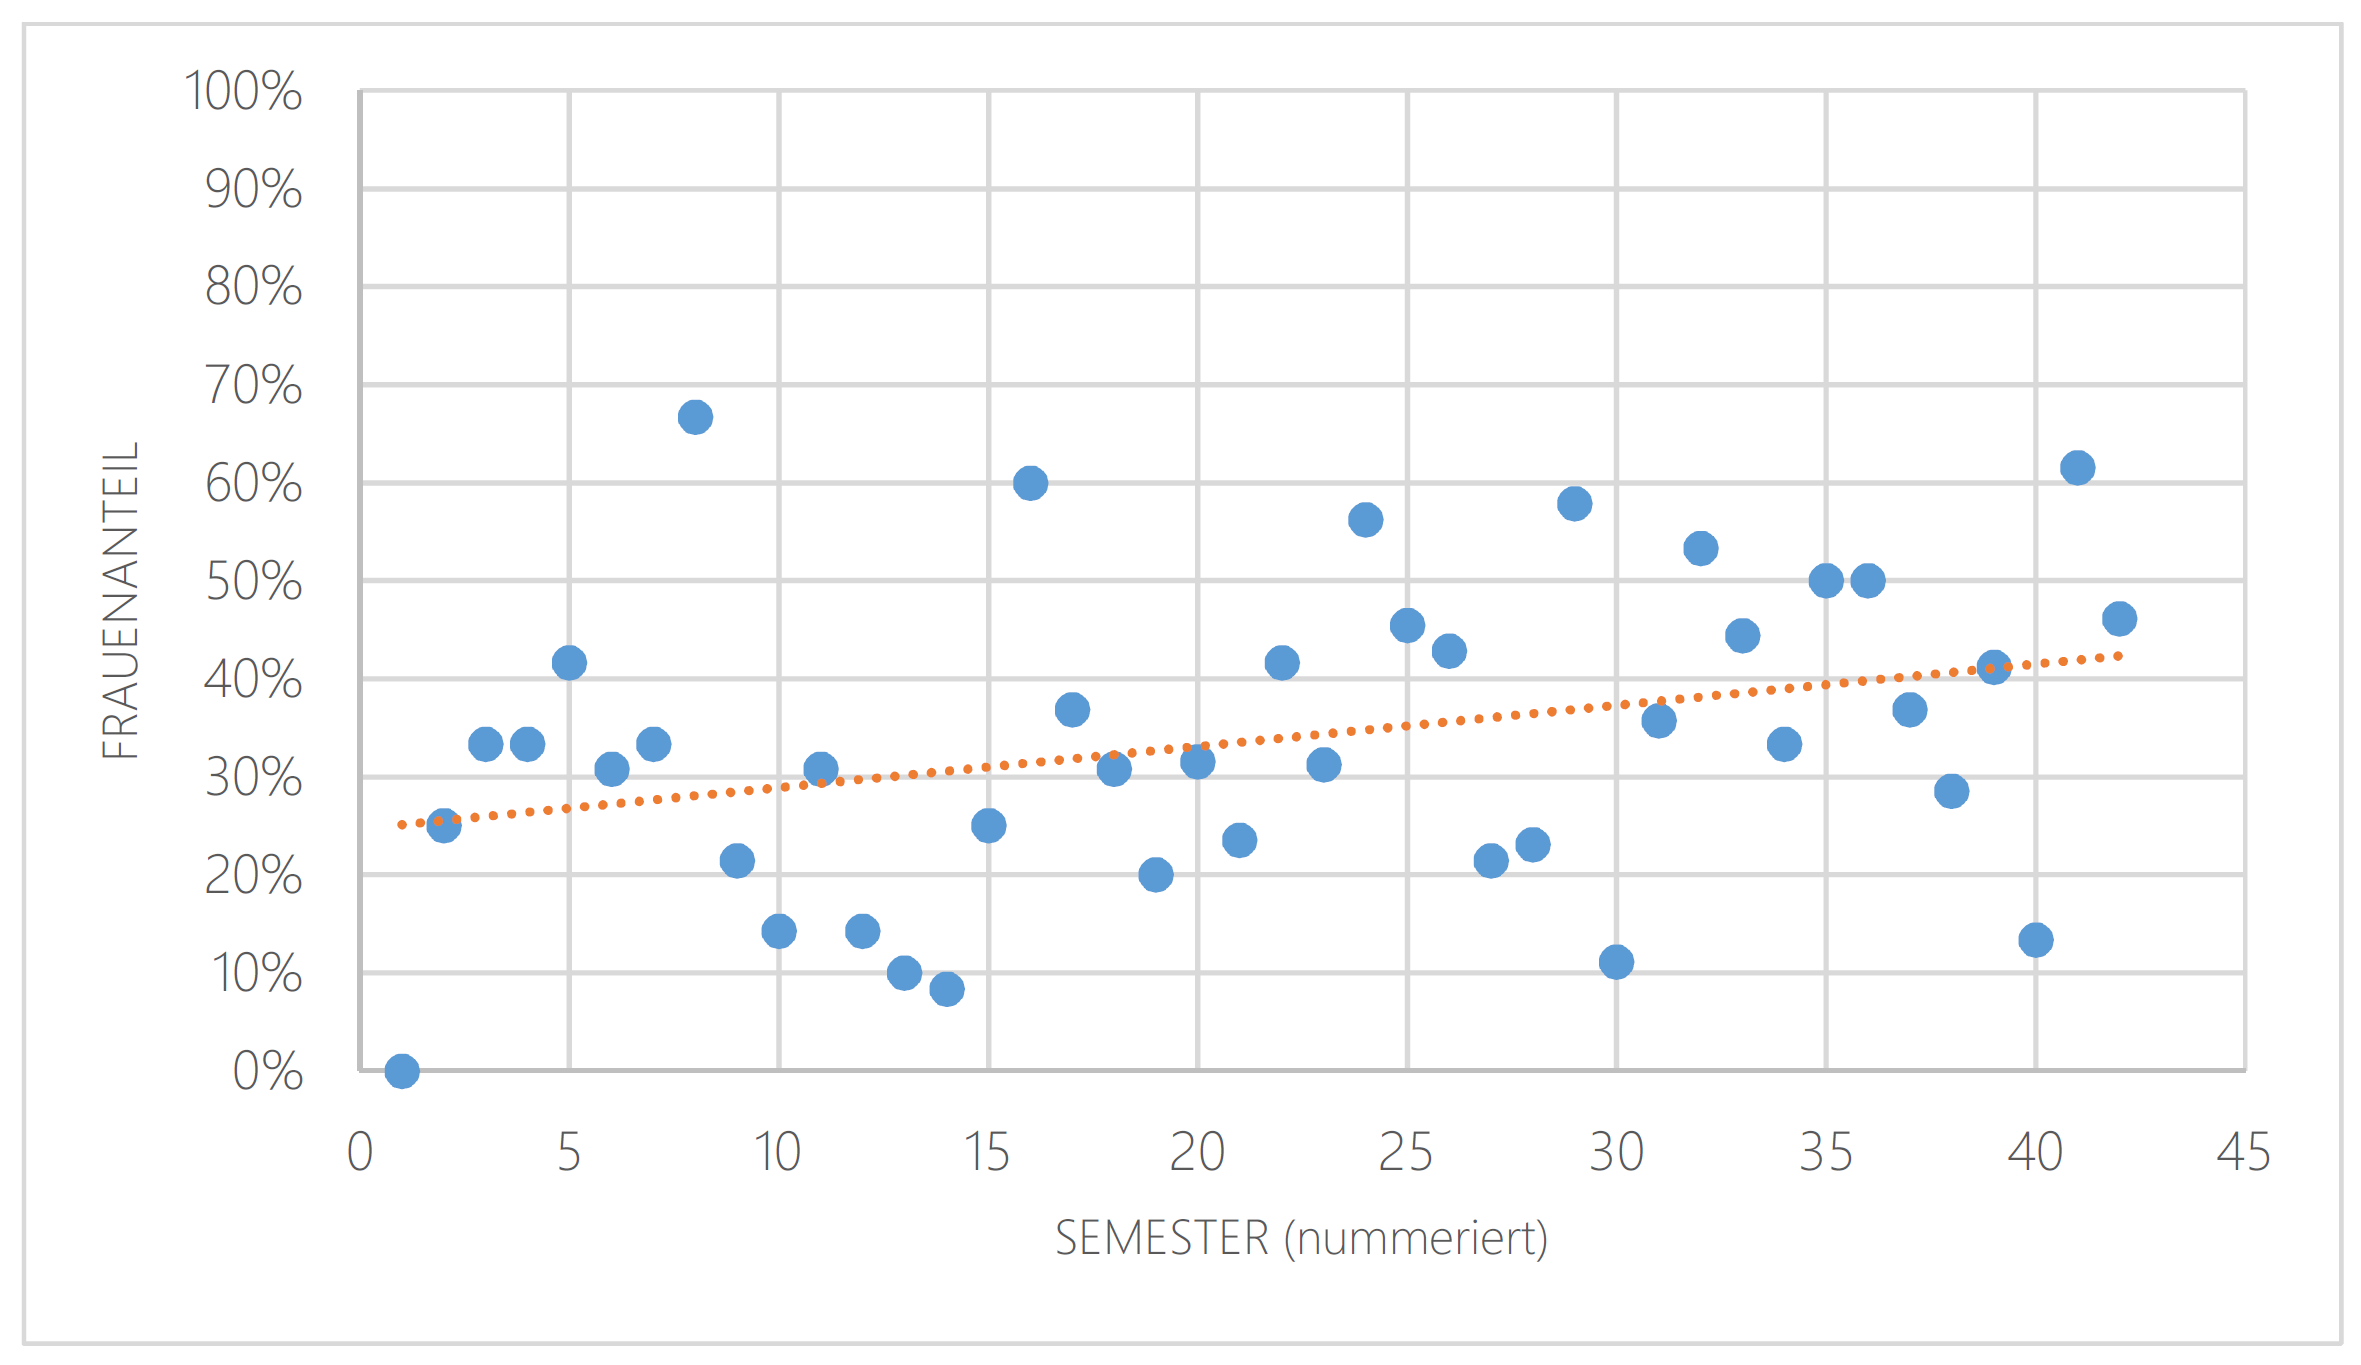
\includegraphics[width=12cm]{img/Abbildung5.png}
\caption{Anteil der Frauen an der Gesamtzahl der ReferentInnen pro
Semester (durchnummeriert, 1 = WS 1997/98)}
\end{figure}

\hypertarget{intern-oder-extern}{%
\subsubsection{Intern oder extern?}\label{intern-oder-extern}}

Interessant ist auch die Frage, aus welchen Einrichtungen die
ReferentInnen der BBK-Vorträge stammen. Für diese Analyse wurde zwischen
Vorträgen unterschieden, die ausschließlich Vortragende mit
IBI-Zugehörigkeit gehalten haben (IBI), Vorträgen, bei denen Personen
aus dem IBI beteiligt waren (IBI anteilig) und Vorträgen, die von
Personen gehalten wurden, bei denen das IBI nicht als Institution
aufgeführt wird (extern). Hier zeigt sich über die Jahre eine klare
Tendenz zu einem verstärkten Anteil von externen ReferentInnen (siehe
Abb. 6).

\begin{figure}
\centering
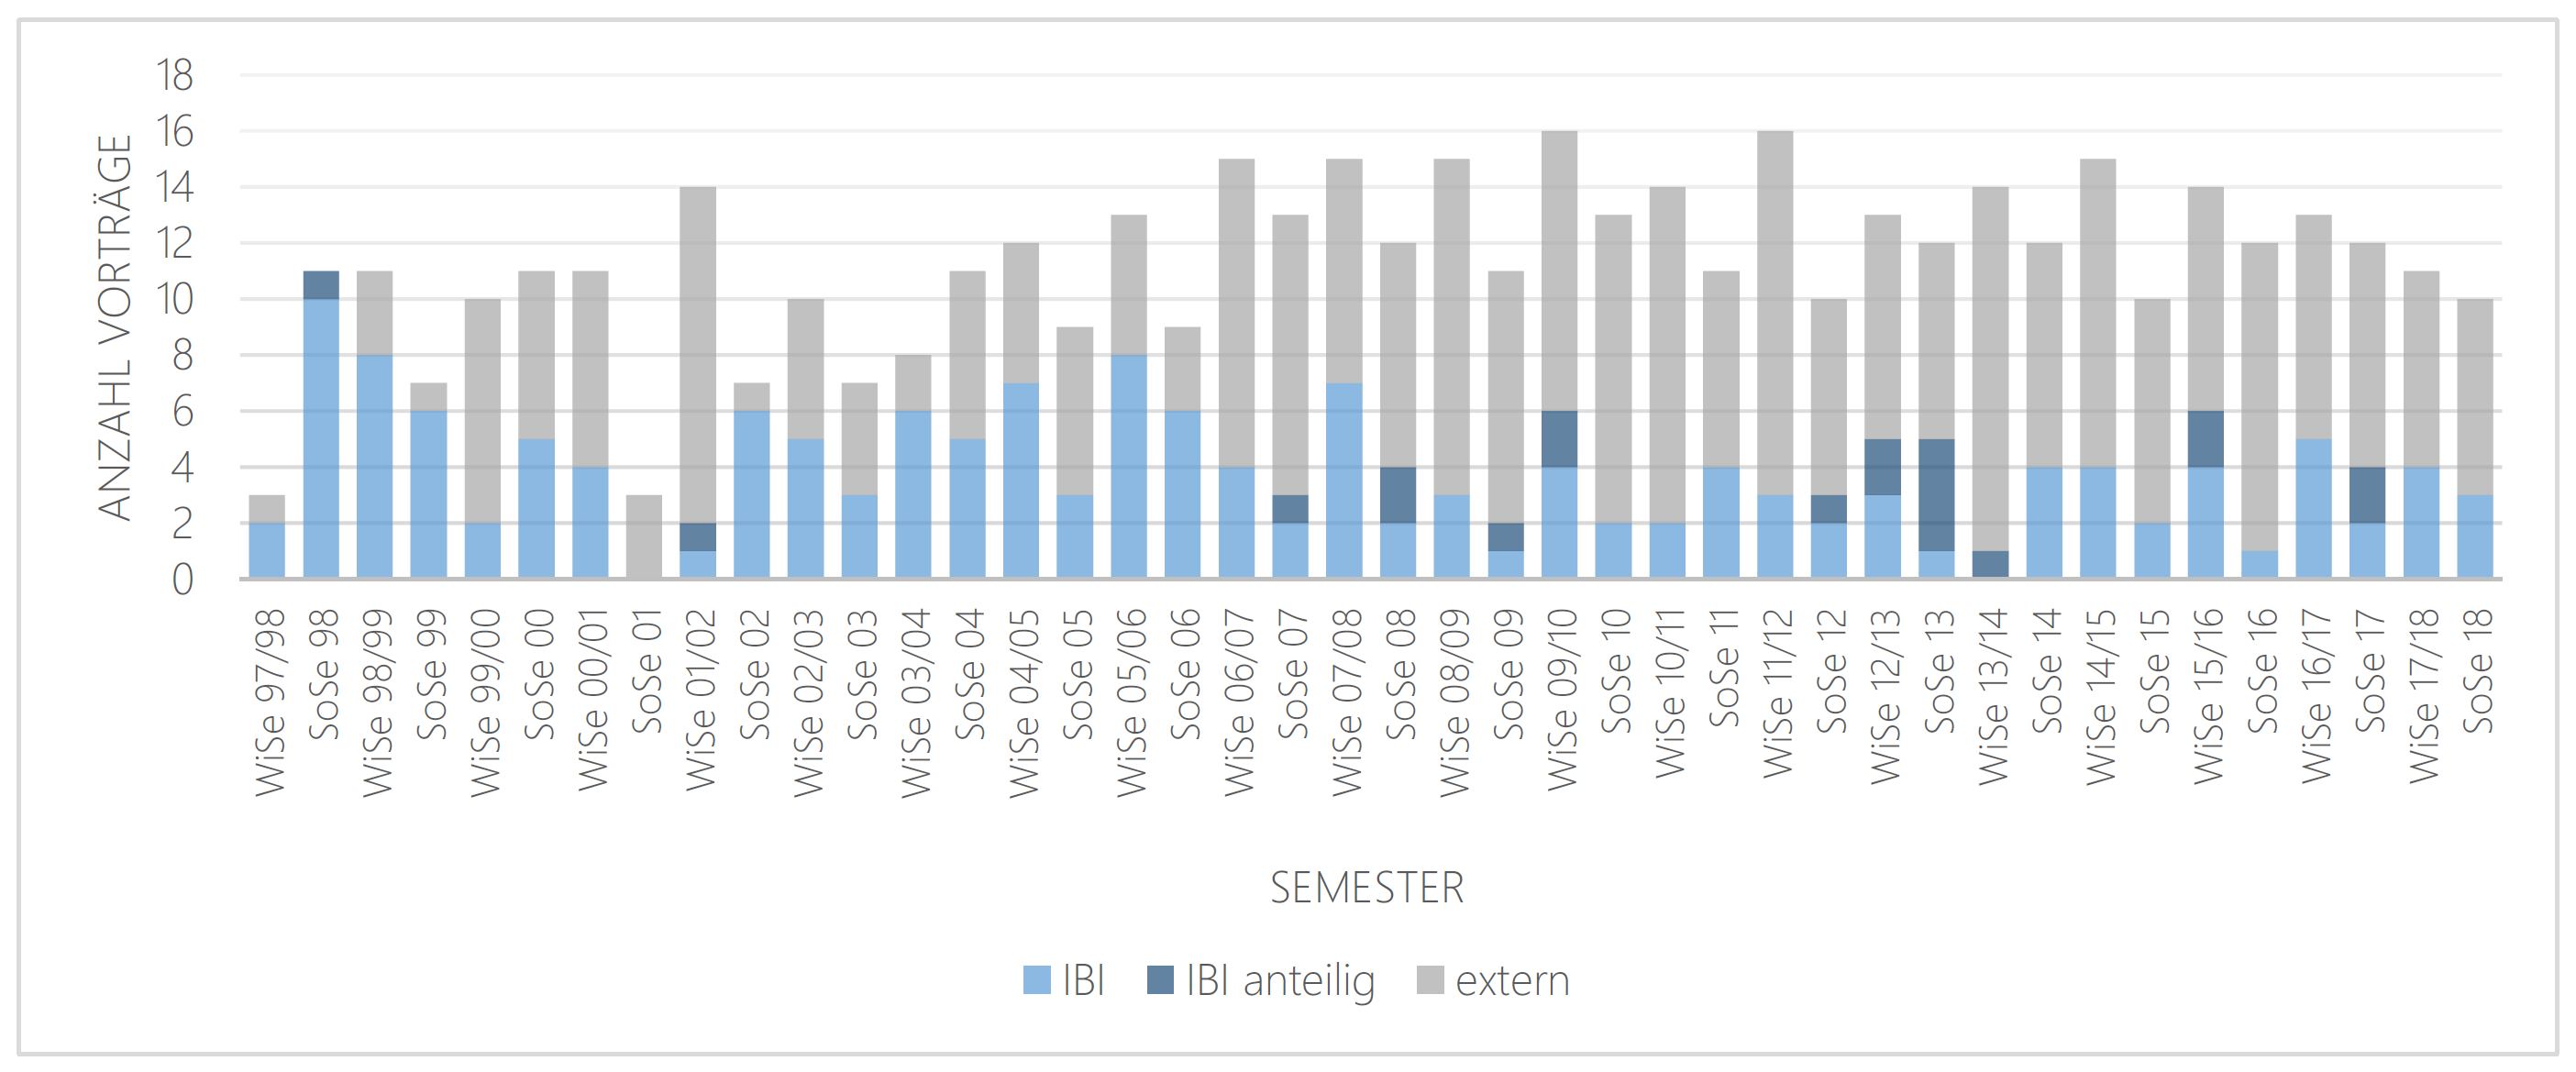
\includegraphics[width=16cm]{img/Abbildung6.png}
\caption{Verhältnis von Vorträgen IBI-intern bzw. extern}
\end{figure}

\hypertarget{internationale-kontakte}{%
\subsubsection{Internationale Kontakte}\label{internationale-kontakte}}

Schon in den frühen Jahren des BBK waren auch regelmäßig internationale
Vortragende zu Gast am IBI: Zwischen 1998 und 2018 haben tatsächlich
ReferentInnen von allen fünf Kontinenten im Rahmen des BBK einen Vortrag
gehalten. Abbildung 7 zeigt die geographische Zuordnung der
internationalen Institutionen, denen die Vortragenden angehörten.
Deutlich wird durch die Grafik auch der Schwerpunkt bei den Kontakten zu
europäischen und nordamerikanischen Einrichtungen, der natürlich durch
die Personalia des Instituts sowie durch die bestehenden Kooperationen
und Partnerschaften (iSchool Organisation; ERASMUS et cetera) entstanden
ist.

\begin{figure}[h!]
\centering
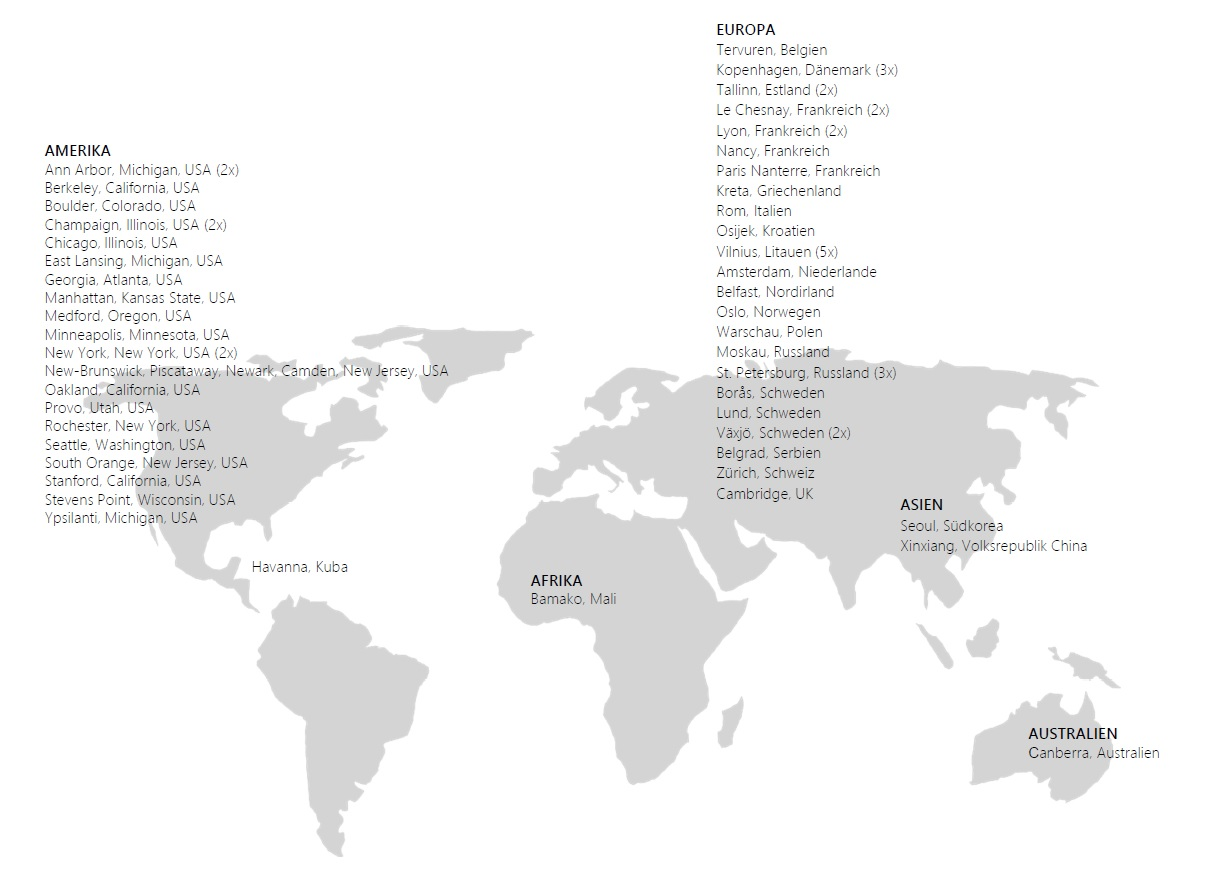
\includegraphics[width=15cm]{img/Abbildung7.jpg}
\caption{Internationale Institutionen zu Gast im BBK}
\end{figure}

Auch an dieser Stelle zeigen sich interessante Entwicklungen im Laufe
der Zeit, die in gewisser Weise die Geschichte des Instituts
widerspiegeln: Während es in den ersten Jahren des BBK verstärkt
Institutionen aus Russland sowie dem Baltikum waren, aus denen
Vortragende aus internationalen Institutionen stammten, lässt sich seit
der Ankunft von Prof.~Michael Seadle eine deutliche Tendenz zu
ReferentInnen aus nordamerikanischen Einrichtungen erkennen.

\hypertarget{themen}{%
\subsection{Themen}\label{themen}}

\hypertarget{entwicklung-uxfcber-die-jahre}{%
\subsubsection{Entwicklung über die
Jahre}\label{entwicklung-uxfcber-die-jahre}}

Das BBK griff immer aktuelle Themen aus der bibliotheks- und
informationswissenschaftlichen Forschung auf. Die Übersicht über die
Vortragstitel der vergangenen 20 Jahre gibt somit auch einen Einblick in
die Entwicklung von Fachdiskursen und Themenfeldern.

Sichtbar wird dies beispielsweise bei der Verfolgung des Begriffes
\emph{Internet} als Teil des Vortragstitels über die Semester hinweg:
Während sich die frühen Vorträge im BBK zum Thema noch mit den
\enquote{Entwicklungen der Informationsrecherche im Internet} (09. Juni
1998) oder der \enquote{inhaltlichen Erschließung des Internets mit
Hilfe von Meta-Daten} (12.01.1999) beschäftigen, geht es am 06.05.2008
bereits um \enquote{Sicherheit und Datenschutz im Internet der Dinge}
und schließlich darum mit \enquote{\emph{Peer-to-Peer} Suchmaschinen}
Informationen im Internet zu vernetzen, Zensur zu verhindern und
Privatsphäre zu sichern (19.06.2012).

Der Suchbegriff \enquote{Bibliothek*} taucht übrigens in insgesamt 164
Titeln von BBK-Vorträgen auf, der Begriff \enquote{Information*} in 67
und der Begriff \enquote{Wissenschaft*} in 74 Titeln. Diese inhaltlichen
Schwerpunkte stellt auch die folgende Wortwolke anschaulich dar, die aus
allen Wörtern erstellt wurde, welche in den BBK-Vortragstiteln zwischen
1998 und 2018 enthalten waren (siehe Abb.~8).

\begin{figure}
\centering
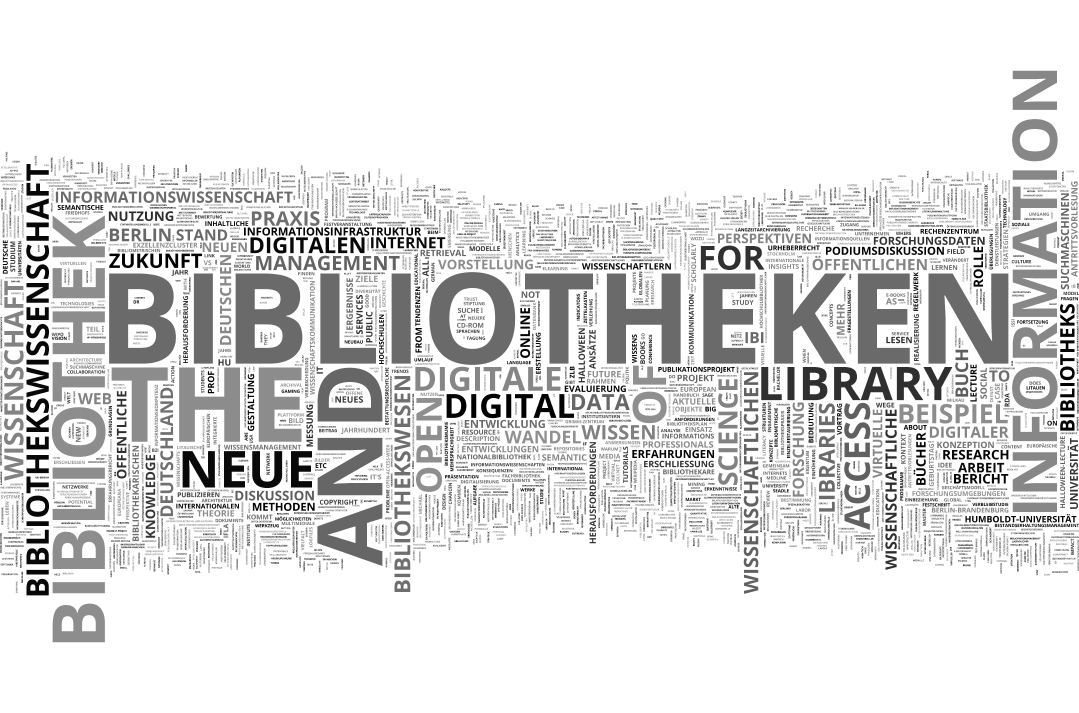
\includegraphics[width=15cm]{img/Abbildung8.png}
\caption{Wortwolke zu den Vortragstiteln des BBK}
\end{figure}

Im BBK wurden aber nicht nur klassische Vorträge gehalten, es fand und
findet auch immer wieder ein reger fachlicher Austausch statt: In
Diskussionsrunden und Panels wurden sowohl interne (Beispielsweise
\enquote{Vorstellung und Diskussion der neuen Entwürfe der
Studienordnungen -- Teil 1-3}; 07.12.2004--11.01.2005) als auch externe
Themen (Beispielsweise \enquote{Wie \glq in \grq ist der/die wissenschaftliche
Bibliothekar/in?}; 25.01.2005) erörtert.

Auch innovative Vortragsformate wurden aufgegriffen: So fand am
27.05.2014 unter der Moderation von Maxi Kindling der erste bibliotheks-
und informationswissenschaftliche Science Slam im Rahmen des BBK statt.
Bereits legendär ist natürlich die \emph{\enquote{Halloween Lecture}}
von Prof.~ Dr.~Eric W. Steinhauer, die am 27.10.2009 mit einem Vortrag
zu friedhofs- und bestattungsrechtlichen Fragestellungen im
Bibliothekswesen ihren Anfang nahm und in den folgenden acht Jahren
unter anderem mit Ausführungen zur \enquote{Theorie und Praxis der
Bibliotheksmumie} sowie zu \enquote{Grundzügen der Vampyrologie für
Bibliothekare} für überfüllte Hörsäle und verängstigte BBK-ZuhörerInnen
sorgte.

Für feierliche Anlässe wurde der Termin des BBK ebenso gerne genutzt:
Neun Antrittsvorlesungen, zwei Verabschiedungen (siehe Tabelle 2) sowie
verschiedene Geburtstagsfeiern und Jubiläen wurden im Laufe der Jahre
als Teil des Berliner Bibliothekswissenschaftlichen Kolloquiums
begangen.

So fand auch im Rahmen des letzten BBK-Termins des Sommersemesters 2018
am 10. Juli 2018 die feierliche akademische Verabschiedung von
Prof.~Michael Seadle, PhD, statt.

\pagebreak

\begin{longtable}[]{@{}lp{8cm}p{5cm}@{}}
\tabularnewline
\toprule
\textbf{Termin} & \textbf{Anlass} & \textbf{Vortragende} \\
\midrule
04.07.2006 & Antrittsvorlesungen & Prof. Dr. Claudia Lux \newline Prof. Dr. Peter Schirmbacher \\
\midrule
24.10.2006 & Akademische Verabschiedung von Prof. Dr. Walther Umstätter & -- \\
\midrule
28.10.2008 & Antrittsvorlesungen der Lehrstühle Digitale Bibliotheken und Wissensmanagement & Prof. Michael Seadle, PhD \newline Prof. Dr. Stefan Gradmann \\
\midrule
10.06.2014 & Antrittsvorlesung: Ein \glq Bibliotheksrecht \grq gibt es natürlich nicht! &
Prof. Dr. Eric W. Steinhauer \\
\midrule
18.11.2014 & Antrittsvorlesung: Big data does not equal big picture & Prof. Dr. Elke Greifeneder \\
\midrule
13.06.2017 & Antrittsvorlesung: Wissenschaft und Bibliothek – vereint im digitalen Wandel? & Prof. Dr. Wolfram Horstmann \\
\midrule
28.11.2017 & Antrittsvorlesung: Das World Wide Web als Ressource für die Wissenschaft & Prof. Dr. Robert Jäschke \\
\midrule
10.07.2018 & Verabschiedung von Prof. Michael Seadle, PhD & -- \\
\bottomrule
\caption{Antrittsvorlesungen und Verabschiedungen im Rahmen des
BBK}
\end{longtable}

\hypertarget{zusammenfassung}{%
\section{Zusammenfassung}\label{zusammenfassung}}

Der vorliegende Beitrag hat einen Blick auf die letzten 20 Jahre des
Berliner Bibliothekswissenschaftlichen Kolloquium (BBK) geworfen,
welches 1998 als Vortragsreihe am Institut für Bibliotheks- und
Informationswissenschaft ins Leben gerufen wurde. Die Auseinandersetzung
mit dem Material bietet dabei nicht nur einen Überblick über die
Entwicklung der Vortragsreihe selbst, sondern ermöglicht auch einen
Einblick in die Geschichte des Instituts, welches in diesem Jahr sein
90-jähriges Jubiläum feiert. Die Vortragenden, ihre Institutionen und
die Titel der Vorträge geben indirekt auch Auskunft über die
personellen, strategischen und inhaltlichen Entwicklungen am Institut
zwischen 1998 und heute.

Neben den oben betrachteten Aspekten lassen sich daher zahlreiche
weitere Fragen an das Datenmaterial stellen: Wie haben sich die
Schwerpunkte bei den behandelten Themen über die Jahre entwickelt,
welche Netzwerke lassen sich im Zusammenhang mit den ReferentInnen
erkennen? Bislang unangetastet blieben auch die Abstracts, welche für
einen größeren Teil der Vorträge zusätzlich vorliegen.

Klar ist, dass das BBK nach wie vor ein wichtiger Teil des Instituts für
Bibliotheks- und Informationswissenschaft ist und noch immer eine
Kommunikationsplattform darstellt, die der fachlichen Weiterbildung für
Studierenden und Lehrende genauso dient wie dem Austausch untereinander
und mit anderen -- sei es auf nationaler oder internationaler Ebene.

\hypertarget{referenzen}{%
\section{Referenzen}\label{referenzen}}

Anderl, Sybille: Trend zum Kollektiv: Die Forschung der vielen, in:
\emph{Frankfurter Allgemeine Zeitung Online} (07.06.2018), URL:
\url{http://www.faz.net/-in2-9auu0} {[}zuletzt abgerufen am 3.10.2018{]}

%autor
\begin{center}\rule{0.5\linewidth}{\linethickness}\end{center}

\textbf{Kirsten Schlebbe} ist wissenschaftliche Mitarbeiterin und
Dozentin am Institut für Bibliotheks- und Informationswissenschaft an
der Humboldt-Universität zu Berlin. Sie hat 2015 ihr Masterstudium am
Institut abgeschlossen. 2016 begann sie ihre Promotion zum digitalen
Informationsverhalten von Klein- und Vorschulkindern bei Prof.~Dr.~Elke
Greifeneder. Seit 2016 betreut sie das Berliner
Bibliothekswissenschaftliche Kolloquium.

\end{document}
